\documentclass[11pt]{article}
 \pdfminorversion=4
\usepackage[utf8]{inputenc}
\usepackage{amsfonts,epsfig}
\usepackage[hyphens]{url}
%\usepackage{hyperref}
\usepackage{breakurl}
\usepackage{comment}
\usepackage{graphicx}
\graphicspath{{./}{./fig/}}
\usepackage{microtype}

\usepackage{natbib}

\linespread{1.25}

\usepackage{relsize}
\usepackage{fancyvrb}
\usepackage{amsmath, amssymb}
%%% Document layout, margins
\usepackage{geometry}
\geometry{letterpaper, textwidth=6.5in, textheight=9in, marginparsep=1em}
%%% Section headings
\usepackage{sectsty}
\usepackage{caption}
\usepackage{subcaption}
\usepackage[normalem]{ulem}
\sectionfont{\sffamily\bfseries\upshape\large}
\subsectionfont{\sffamily\bfseries\upshape\normalsize}
\subsubsectionfont{\sffamily\mdseries\upshape\normalsize}
\makeatletter
\renewcommand\@seccntformat[1]{\csname the#1\endcsname.\quad}

\makeatletter
\def\@maketitle{%
  \begin{center}%
  \let \footnote \thanks
    {\large \@title \par}%
    {\normalsize
      \begin{tabular}[t]{c}%
        \@author
      \end{tabular}\par}%
    {\small \@date}%
  \end{center}%
}
\makeatother


\title{\bf R-squared for Bayesian regression models\footnote{To appear in {\em The American Statistician}.
  We thank Frank Harrell and Daniel Jeske for helpful comments and the National Science Foundation,
  Office of Naval Research, Institute for Education Sciences, Defense Advanced Research Projects Agency, and Sloan Foundation
  for partial support of this work.}\vspace{.1in}}
\author{Andrew Gelman\footnote{Department of Statistics and Department of Political Science, Columbia University.}
  \and Ben Goodrich\footnote{Institute for Social and Economic Research and Policy, Columbia University.}
  \and Jonah Gabry$^\ddagger$
\and Aki Vehtari\footnote{Department of Computer Science, Aalto University.}\vspace{.1in}}
\date{1 Nov 2018\vspace{-.1in}}
\begin{document}\sloppy
\maketitle
\thispagestyle{empty}

\begin{abstract}
The usual definition of $R^2$ (variance of the predicted values divided by the
variance of the data) has a problem for Bayesian fits, as the numerator can be
larger than the denominator.  We propose an alternative definition similar to
one that has appeared in the survival analysis literature:  the variance of the
predicted values divided by the variance of predicted values plus the expected variance 
of the errors.
\end{abstract}

\section{The problem}

Consider a regression model of outcomes $y$ and predictors $X$ with predicted
values $\mbox{E}(y|X,\theta)$, fit to data $(X,y)_n, \, n=1,\ldots,N$.  Ordinary
least squares yields an estimated parameter vector $\hat{\theta}$
with predicted values $\hat{y}_n = \mbox{E}(y | X_n, \hat{\theta})$ and residual
variance $V_{n=1}^N \,\hat{y}_n$, where we are using the notation,
%
$$
V_{n=1}^N \, z_n = \frac{1}{N-1}\sum_{n=1}^N (z_n - \bar{z})^2, \mbox{ for any vector }z.
$$
%
The proportion of variance explained,
%
\begin{equation}\label{rsq1}
\mbox{classical } R^2 = \frac{V_{n=1}^N \,\hat{y}_n}{V_{n=1}^N \,y_n},
\end{equation}
%
is a commonly used measure of model fit, and there is a long literature on
interpreting it, adjusting it for degrees of freedom used in fitting the model,
and generalizing it to other settings such as hierarchical models; see, for example, \cite{Xu2003}
and \cite{GelmanPardoe2006}.

Two challenges arise in defining $R^2$ in a Bayesian context.  The first is the desire to reflect posterior uncertainty in the coefficients, which should remove or at least reduce the overfitting problem of least squares.  Second, in the presence of strong prior information and weak data, it is possible for the fitted variance, $V_{n=1}^N \,\hat{y}_n$  to be higher than total variance, $V_{n=1}^N \,y_n$, so that the classical formula (\ref{rsq1}) can yield an $R^2$ greater than 1 \citep{Tjur2009}.  In the present paper we propose a generalization that has a Bayesian interpretation as a variance decomposition.


\section{Defining $R^2$ based on the variance of estimated prediction errors}

Our first thought for Bayesian $R^2$ is simply to use the posterior mean
estimate of $\theta$ to create Bayesian predictions $\hat{y}_n$
and then plug these into the classical formula \eqref{rsq1}.
This has two problems:  first,
it dismisses uncertainty to use a point estimate in Bayesian computation;
and, second, the ratio as thus defined can be greater than 1.  When
$\hat{\theta}$ is estimated using ordinary least squares, and assuming the
regression model includes a constant term, the numerator of \eqref{rsq1} is less
than or equal to the denominator by definition; for general estimates, though, there is
no requirement that this be the case, and it would be awkward to say that a
fitted model explains more than 100\% of the variance.

\begin{figure}
\centerline{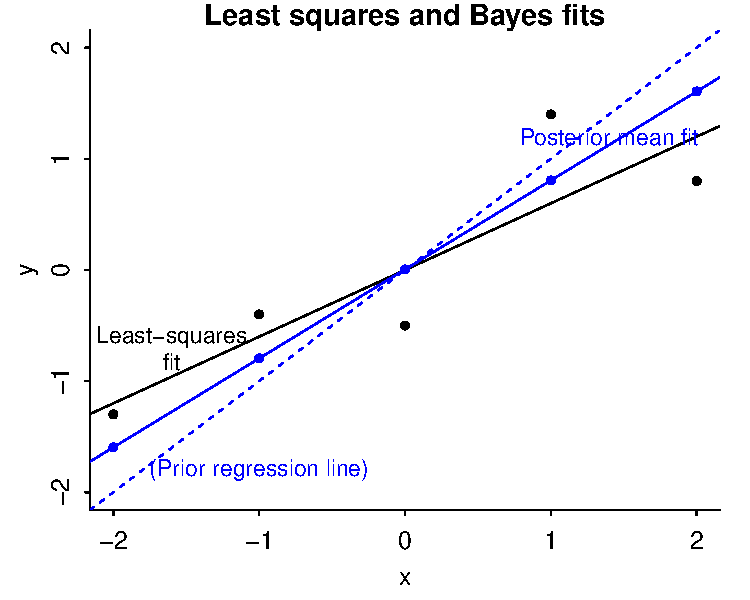
\includegraphics[width=.5\textwidth]{rsquared1a.pdf}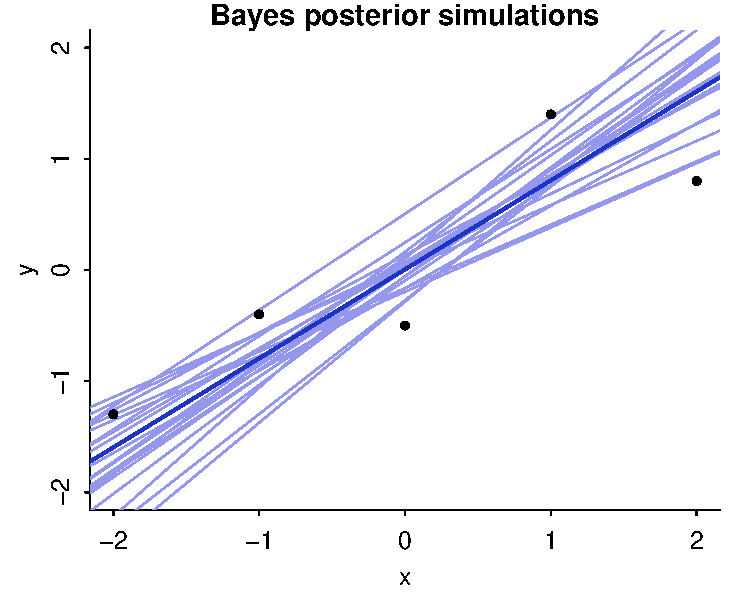
\includegraphics[width=.5\textwidth]{rsquared1b.pdf}}
\vspace{-.1in}
\caption{\em Simple example showing the challenge of defining $R^2$ for a fitted
Bayesian model.  {\em Left plot:}  data, least-squares regression line, and
fitted Bayes line, which is a compromise between the prior and the least-squares
fit.  The standard deviation of the fitted values from the Bayes model (the blue
dots on the line) is greater than the standard deviation of the data, so the
usual definition of $R^2$ will not work.  {\em Right plot:}  posterior mean
fitted regression line along with 20 draws of the line from the posterior
distribution.  To define the posterior distribution of Bayesian $R^2$ we compute equation
\eqref{rsq3} for each posterior simulation draw.}
\label{rsquared1}
\end{figure}

To see an example where the simple $R^2$ would be inappropriate, consider the model
$y = \alpha + \beta x+\mbox{error}$
with a strong prior on $(\alpha,\beta)$ and only a few data points.
Figure~\ref{rsquared1}a shows data and the least-squares regression line, with
$R^2$ of 0.77.  We then do a Bayes fit with informative priors
$\alpha \sim \mbox{N}(0,0.2^2)$ and $\beta \sim \mbox{N}(1,0.2^2)$.
The standard deviation of the fitted values from the Bayes model is 1.3, while
the standard deviation of the data is only 1.08, so the square of this
ratio---$R^2$ as defined in \eqref{rsq1}---is greater than 1.
Figure~\ref{rsquared1}b shows the posterior mean fitted regression line along
with 20 draws of the line $y = \alpha + \beta x$ from the fitted posterior
distribution of $(\alpha,\beta)$.
% \footnote{Code for this example is available at \url{https://github.com/jgabry/bayes_R2}.}
% I removed this link because (a) I don't want us to have the responsibility of maintaining it, (b) it would need to be updated anyway to work with our new definition, and (c) the reviewer had a problem running the code.

Here is our proposal.  First, instead of using point predictions $\hat{y}_n$, we use expected values conditional on the unknown parameters,
$$y^{\rm pred}_n=\mbox{E}(\tilde{y}|X_n,\theta),$$
where $\tilde{y}$ represents a future observation from the model. 
For a linear model, $y^{\rm pred}_n$ is simply the linear predictor, $X_n\beta$; for a generalized linear model it is the linear predictor transformed to the data scale.
The posterior distribution of $\theta$ induces a posterior predictive distribution for $y^{\rm pred}$.

Second, instead of working with \eqref{rsq1} directly, we define $R^2$ explicitly based on the distribution of future data $\tilde{y}$, using the following variance decomposition for the denominator:
%
\begin{equation}\label{rsq2}
\mbox{alternative } R^2 = \frac{\mbox{Explained variance}}{\mbox{Explained variance} + \mbox{Residual variance}} = \frac{{\rm var}_{\rm fit}}{{\rm var}_{\rm fit} + {\rm var}_{\rm res}},
\end{equation}
where
\begin{eqnarray}
\nonumber  {\rm var}_{\rm fit} = V_{n=1}^N  \mbox{E}(\tilde{y}_n|y) = V_{n=1}^N \,y^{\rm pred}_n && \!\!\!\!\!\!\!\! \mbox{is the variance of the modeled predictive means, and} \\
\nonumber  {\rm var}_{\rm res}=\mbox{E}( V_{n=1}^N (\tilde{y}_n - y^{\rm pred}_n)|y) && \!\!\!\!\!\!\!\! \mbox{is the modeled residual variance}.
\end{eqnarray}
This first of these quantites is the variance among the expectations of the new data; the second term is the expected variance for new residuals, in both cases assuming the same predictors $X$ as in the observed data. We are following the usual practice in regression to model the outcomes $y$ but not the predictors $X$. 

Both variance terms can be computed using posterior quantities from the fitted model:  ${\rm var}_{\rm fit}$ is determined based on $y^{\rm pred}$ which is a function of model parameters (for example,  $y^{\rm pred}_n=X_n\beta$ for linear regression and $y^{\rm pred}_n=\mbox{logit}^{-1}(X_n\beta)$ for logistic regression), and ${\rm var}_{\rm res}$ depends on the modeled probability distribution; for example, ${\rm var}_{\rm res}= \sigma^2$ for simple linear regression and ${\rm var}_{\rm res}= \frac{1}{N}\sum_{n=1}^N (\pi_n(1-\pi_n))$ for logistic regression.

%For least squares regression, (\ref{rsq2}) reduces to (\ref{rsq1}):  the two expressions only differ in their denominator, and with least squares the estimated residual standard deviation $\hat{\sigma}$ is computed using the variance of the residuals $r$.
By construction, the ratio \eqref{rsq2} is always between $0$ and $1$, no matter what procedure is used to construct the estimate
$y^{\rm pred}$.
Versions of \eqref{rsq2} have appeared in the survival analysis
literature \citep{KentOquigley1988, ChoodariRoystonParmar2010},
where it makes sense to use expected rather than observed data variance
in the denominator, as this allows one to compute a measure of explained variance that is completely independent of the censoring distribution in time-to-event models.  Our motivation is slightly different but the same
mathematical principles apply, and our measure could also be extended to nonlinear models.


\begin{figure}
\centerline{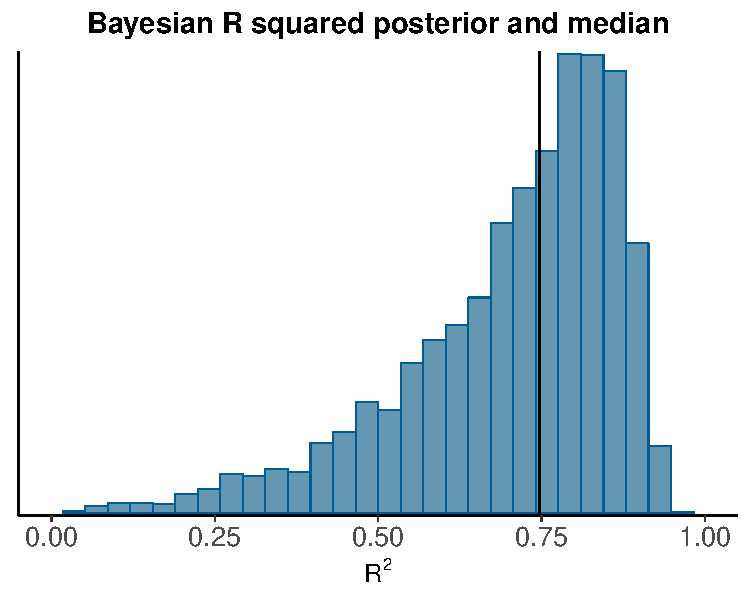
\includegraphics[width=.5\textwidth]{bayesr2post.pdf}}
\vspace{-.1in}
\caption{\em The posterior distribution of Bayesian $R^2$ for the simple example shown in Figure~\ref{rsquared1} computed using equation \eqref{rsq3} for each posterior simulation draw.}
\label{bayesr2post}
\end{figure}

In Bayesian inference, instead of a point estimate $\hat{\theta}$, we have
a set of posterior simulation draws, $\theta^s, \,s=1,\ldots,S$.
For each $\theta^s$, we can compute the vector of predicted values
$y^{{\rm pred}\,s}_n = \mbox{E}(y | X_n, \theta^s)$ and the expected residual variance
$\mbox{var}_{\rm res}^s$, and thus the proportion of variance explained is,
%
\begin{equation}\label{rsq3}
\mbox{Bayesian } R^2_s = 
	\frac{V_{n=1}^N \,y^{{\rm pred}\,s}_n} {V_{n=1}^N \,y^{{\rm pred}\,s}_n  +\mbox{var}_{\rm res}^s},
      \end{equation}
      where $\mbox{var}_{\rm res}^s=(\sigma^2)^s$ for a linear regression model with equal variances.
%
%We could then summarize this by its posterior mean or median, for example.

%An alternative to \eqref{rsq3} is the ratio of sums of squares, $\sum_{n=1}^N (y^{{\rm pred}\,s}_n)^2\big/\sum_{n=1}^N (\tilde{y}_n^s)^2$, where $\tilde{y}$ is distributed according to the posterior predictive distribution.  When computed in this way, each Bayesian $R^2_s$ is the ratio of the sum of squares of a posterior draw of the conditional mean to the sum of squares of a draw from the posterior predictive distribution. However, although equal asymptotically to \eqref{rsq3}, in practice the denominator of this new expression can be smaller than the numerator due to Monte Carlo variation and so the resulting ratio can be greater than 1, which seems contrary to the goal of $R^2$ to partition variance in the data.


For linear regression and generalized linear models, expression (\ref{rsq3}) can be computed using the \verb#posterior_linpred# function in the {\tt rstanarm}
package and a few additional lines of code, as we demonstrate in the appendix, or see \cite{br2} for further development.
For the example in Figure~\ref{rsquared1}, we display the posterior distribution of $R^2$ in Figure~\ref{bayesr2post}; this distribution has median 0.75, mean 0.70, and standard deviation 0.17.
% In comparison, if we were to replace the denominator of \eqref{rsq3} by $V_{n=1}^N \,y_n$, we would get a median $R^2$ of 1.44. 

\section{Discussion}
$R^2$ has well-known problems as a measure of model fit, but it can be a handy quick summary for linear regressions and generalized linear models \citep[see, for example,][]{HuPaltaShao2006}, and we would like to produce it by default when fitting Bayesian regressions.  Our preferred solution is to use \eqref{rsq3}:  predicted variance divided by predicted variance plus error variance.   This measure is model based:  all variance terms come from the model, and not directly from the data.

A new issue then arises, though, when fitting a set of a models to a single dataset.  Now that the denominator of $R^2$ is no longer fixed, we can no longer interpret an increase in $R^2$ as a improved fit to a fixed target.  We think this particular loss of interpretation is necessary:  from a Bayesian perspective, a concept such as ``explained variance'' can ultimately only be interpreted in the context of a model.  The denominator of \eqref{rsq3} can be interpreted as an estimate of the expected variance of predicted future data from the model under the assumption that the predictors $X$ are held fixed; alternatively the predictors can be taken as random, as suggested by \cite{Helland1987} and \cite{Tjur2009}.  In either case, we can consider our Bayesian $R^2$ as a data-based estimate of the proportion of variance explained for new data. If the goal is to see continual progress of the fit to existing data, one can simply track the decline in the expected error variance, $\sigma^2$.

%We have implemented our Bayesian $R^2$ by default in our Bayesian regression package {\tt rstanarm}, not just for linear regression but also for generalized linear models; see the appendix for a generalized version of the \verb#bayes_R2# function. The concept of ``explained variance'' makes most sense for linear models with equal variance, but given that we can essentially compute $R^2$ for free, we might as well do so.  An alternative is to summarize residual error on the log-probability scale, in which case we recommend using approximate leave-one-out cross-validation \citep{VehtariGelmanGabry2017}, which can be done using the {\tt loo} function within {\tt rstanarm}. If desired, changes in expected log-probability scores can be converted back to an $R^2$ scale as discussed by \cite{Nagelkerke1991}.

Another issue that arises when using $R^2$ to evaluate and compare models is overfitting.  As with other measures of predictive model fit, overfitting should be less of an issue with Bayesian inference because averaging over the posterior distribution is more conservative than taking a least-squares or maximum likelihood fit, but predictive accuracy for new data will still on average be lower, in expectation, than for the data used to fit the model \citep{GelmanHwangVehtari2014}.
%The \verb#bayes_R2# function also takes a  {\tt newdata} argument that can be used in the case that new or held-out data are actually available, but otherwise to correct for that bias one might want to replace $V_{n=1}^N \,e_n^s$ in the denominator of \eqref{rsq3} by its expectation for new data, or more generally
One could construct an overfitting-corrected $R^2$ in the same way that is done for log-score measures via cross-validation \citep{VehtariGelmanGabry2017}. In the present paper we are trying to stay close to the sprit of the original $R^2$ in quantifying the model's fit to the data at hand.



%: references (see separate bayes_R2.bib file)
\bibliography{bayes_R2}
\bibliographystyle{chicago}

%: appendix
\clearpage
\section*{Appendix}

This simple version of the \verb#bayes_R2# function works with
Bayesian linear regressions fit using the
\verb#stan_glm# function in the {\tt rstanarm} package.

%
\vspace{-\baselineskip}
\begin{quotation}
\noindent
\begin{small}
\begin{verbatim}
# Compute Bayesian R-squared for linear models.
#
# @param fit A fitted linear or logistic regression object in rstanarm
# @return A vector of R-squared values with length equal to
#      the number of posterior draws.
#
bayes_R2 <- function(fit) {
  y_pred <- rstanarm::posterior_linpred(fit)
  var_fit <- apply(y_pred, 1, var)
  var_res <- as.matrix(fit, pars = c("sigma"))^2
  var_fit / (var_fit + var_res)
}

## Example from Figure 1 of the paper
x <- 1:5 - 3
y <- c(1.7, 2.6, 2.5, 4.4, 3.8) - 3
xy <- data.frame(x,y)

## Bayes fit with strong priors
library("rstanarm")
fit_bayes <- stan_glm(y ~ x, data = xy,
  prior_intercept = normal(0, 0.2, autoscale = FALSE),
  prior = normal(1, 0.2, autoscale = FALSE), 
  prior_aux = NULL)

## Compute Bayesian R2
rsq_bayes <- bayes_R2(fit_bayes)
hist(rsq_bayes)
print(c(median(rsq_bayes), mean(rsq_bayes), sd(rsq_bayes)))
\end{verbatim}
\end{small}
\end{quotation}
Expanding the code to work for other generalized linear models requires some additional steps, including setting \verb#transform=TRUE# in the call to
\verb#posterior_linpred# (to apply the inverse-link function to the linear
predictor), the specification of the formula for $\mbox{var}_{\rm res}$ for each distribution class, and code to accomodate multilevel models fit using \verb#stan_glmer#.

\end{document}
